\documentclass[12pt]{report}

% Packages
\usepackage{amsmath}
\usepackage{graphicx}
\usepackage{hyperref}
\usepackage{caption}
\usepackage{subcaption}
\usepackage{geometry}
\usepackage{fancyhdr}
\usepackage{float}
\usepackage{titlesec}

% Page settings
\geometry{a4paper, margin=1in}

% Header and footer
\pagestyle{fancy}
\fancyhf{}
\fancyhead[L]{\leftmark}
\fancyfoot[C]{\thepage}

% Title format
\titleformat{\chapter}[block]{\normalfont\Large\bfseries}{\thechapter.}{1em}{}

% Title page
\title{EEG Controlled Robotic Arm \\ \large{BME 1317 Project}}
\author{Gangfeng Hu \and Quanyu Chen \and Yumeng Wang}
\date{\today}

\begin{document}

% Title page
\maketitle

% Abstract
\begin{abstract}
This report presents the development and implementation of an EEG (Electroencephalography) controlled robotic arm. The project utilizes EEG signals to control a robotic arm, aiming to achieve tasks through brain-computer interface technology. The report details the research background, materials used, system workflow, and current challenges faced during the project's iterations.
\end{abstract}

% Table of contents
\tableofcontents
% \listoffigures
% \listoftables

% Main content

\chapter{Introduction}
Individuals with extremity disabilities face significant challenges in performing everyday tasks, often relying on assistive devices that can be cumbersome and unintuitive. For instance, those with advanced Parkinson's disease or congenital upper limb absence have a significant need for assistive technology to perform daily tasks.

EEG (Electroencephalography) is a method to record the spontaneous electrical activity of the brain. When the brain is active, postsynaptic potentials from numerous neurons are summed up, and these electric fields are conducted to the scalp's surface. Electrodes pick up these signals and transmit them to an electroencephalogram machine. Brain waves are divided into frequency bands such as Delta, Theta, Alpha, Beta, and Gamma, each associated with specific brain states or activities.

The 10-20 system is a standardized method of electrode placement for EEG recording, ensuring consistency with brain anatomy. This system improves the comparability and reproducibility of EEG data.

The primary objective is to control a robotic arm using EEG signals. This involves capturing brain activity, processing the signals, and translating them into commands for the robotic arm. By leveraging brain-computer interface (BCI) technology, the project aims to provide a more natural and intuitive method of control for users with extremity disabilities.

\chapter{Method}
\section{Materials}
\subsection{EEG Acquisition Device}
The project uses an EEG acquisition device based on the OpenBCI open-source platform, including a Cyton Board, electrodes, and a headwear. The Cyton Board processes and sends the data to a graphical user interface (GUI).

% \begin{figure}[H]
%     \centering
%     \includegraphics[width=0.5\textwidth]{eeg_cap.jpg} % Replace with actual image path
%     \caption{8-channel EEG cap}
%     \label{fig:eeg_cap}
% \end{figure}

\subsection{Robotic Arm}
The Songjia Am1 robotic arm is equipped with six steering engines and supports serial port transmission. Each engine has an individual value of Pulse Width Modulation (PWM), controlled by an STM32 circuit board through C code.

% \begin{figure}[H]
%     \centering
%     \includegraphics[width=0.5\textwidth]{robotic_arm.jpg} % Replace with actual image path
%     \caption{Songjia AM1 Robotic Arm}
%     \label{fig:robotic_arm}
% \end{figure}

\section{System Workflow}
The system consists of five basic stages: signal acquisition, preprocessing, feature extraction, classification, and robotic arm control. 

% \begin{figure}[H]
%     \centering
%     \includegraphics[width=0.8\textwidth]{workflow.jpg} % Replace with actual image path
%     \caption{Flowchart of EEG processing}
%     \label{fig:workflow}
% \end{figure}

\section{Version Iteration}
\subsection{Version 1}
The first version focuses on acquiring signals and enabling real-time interaction between the devices. Specific commands like blinking are used to perform simple tasks.

\subsubsection{EEG Signal Acquisition and Identification}
The setup utilizes the OpenBCI platform with a Cyton board. Signals are processed every 300 ms, and significant peaks from muscle activity during blinking are detected using a threshold method.

\subsubsection{Robotic Arm Control and Communication}
The robotic arm is programmed to perform basic tasks, and real-time communication is established between the EEG device and the arm.

\subsection{Version 2}
The second version implements more commands using actions like blinking and head movements for tasks like remote object retrieval.

\subsubsection{EEG Signal Preprocessing}
Signals are denoised and filtered using the EEGLAB clean raw data algorithm.

\subsubsection{Eye Tracking}
Eye movements are tested for significant changes in EEG signals to control the robotic arm.

\subsection{Version 2.5}
In order to iteratively improve the system, a version 2.5 was introduced to enhance the real-time control of the robotic arm using EEG signals and eye tracking. 
We plan to use SSVEP (Steady-State Visually Evoked Potential) to control the robotic arm in real-time, which is a promising method for BCI applications and has a better robustness and accuracy compared to other methods. 

\subsection{Version 3}
The final version aims to enable the robotic arm to mimic human arm movements using motor imagery.


\chapter{Results}
\section{Version 1 Implementation}
In the first version, the system successfully acquired EEG signals and translated them into commands for the robotic arm. Simple tasks were performed using blinking as a control signal.

\begin{figure}[h]
    \centering
    \includegraphics[width=0.8\textwidth]{../imgs/workflow.png}
    \caption{Workflow of EEG processing}
    \label{fig:workflow}
\end{figure}

As shown in Figure \ref{fig:workflow}, the system workflow consists of five main parts: signal acquisition, preprocessing 
(which has been encapsulated by the OpenBCI GUI), feature extraction, classification (which is implemented in EEGCache), and robotic arm control. 
The EEG signals are acquired using the OpenBCI Cyton board, preprocessed in the OpenBCI GUI, and then sent to the feature extraction and classification modules. 
The classification results are used to control the robotic arm. 

\section{Version 2 Implementation}
To achieve the original goal of controlling the robotic arm to pick up objects, the system was improved in version 2. 
It is found that when knocking different channels of the EEG cap, the EEG signals will change significantly. 
Therefore, the system was designed to control the robotic arm to move by knocking different channels of the EEG cap. 
What's more, we use eye-blinking to control the robotic arm to catch the object.

During the 4-week summer term, we have not finished the implementation of the version 2.5 and version 3. 
However, we have made some progress in the implementation of the version 2.5. 
We have implemented the screen of SSVEP, which can display the flickering images. 
But we have not finished the implementation of the SSVEP classification algorithm.

\chapter{Discussion and Conclusion}
\section{Current Challenges}
\subsection{Version 2.5 Challenges}
Designing a system for real-time screen-EEG-arm control is complex. Applying an appropriate model for real-time classification is challenging, and there is a lack of fully public related work.

\subsection{Version 3 Challenges}
Achieving high accuracy in motor imagery classification is difficult. The highest accuracy achieved so far is around 72.15% with MSRTNet.

\section{Discussion}
The development of an EEG-controlled robotic arm offers significant potential for assisting individuals with extremity disabilities. While the project has made substantial progress, further research and refinement are needed to improve real-time classification accuracy and overall system performance. Future work will focus on enhancing the robustness of the system and exploring additional applications of brain-computer interface technology.

\chapter{Contributions of Group Members}
During this summer term, all of us were dedicated to the project, and have great help of the implementation of the project.
\begin{itemize}
    \item Gangfeng Hu: Design of the system workflow and the implementation of EEG signal preprocessing.
    \item Quanyu Chen: Responsible for the implementation of the EEG signal acquisition and the robotic arm control.
    \item Yumeng Wang: Responsible for the search of the background knowledge, implementation of the arm control, and the implementation of the SSVEP screen.
\end{itemize}


In the end, we would like to thank our instructor, Prof. Ren and Prof. Cui, for their guidance and support during the project.
And we would like to thank our TA, Mr. Li, for his help in the implementation of the project.

\end{document}